\documentclass[1p]{elsarticle_modified}
%\bibliographystyle{elsarticle-num}

%\usepackage[colorlinks]{hyperref}
%\usepackage{abbrmath_seonhwa} %\Abb, \Ascr, \Acal ,\Abf, \Afrak
\usepackage{amsfonts}
\usepackage{amssymb}
\usepackage{amsmath}
\usepackage{amsthm}
\usepackage{scalefnt}
\usepackage{amsbsy}
\usepackage{kotex}
\usepackage{caption}
\usepackage{subfig}
\usepackage{color}
\usepackage{graphicx}
\usepackage{xcolor} %% white, black, red, green, blue, cyan, magenta, yellow
\usepackage{float}
\usepackage{setspace}
\usepackage{hyperref}

\usepackage{tikz}
\usetikzlibrary{arrows}

\usepackage{multirow}
\usepackage{array} % fixed length table
\usepackage{hhline}

%%%%%%%%%%%%%%%%%%%%%
\makeatletter
\renewcommand*\env@matrix[1][\arraystretch]{%
	\edef\arraystretch{#1}%
	\hskip -\arraycolsep
	\let\@ifnextchar\new@ifnextchar
	\array{*\c@MaxMatrixCols c}}
\makeatother %https://tex.stackexchange.com/questions/14071/how-can-i-increase-the-line-spacing-in-a-matrix
%%%%%%%%%%%%%%%

\usepackage[normalem]{ulem}

\newcommand{\msout}[1]{\ifmmode\text{\sout{\ensuremath{#1}}}\else\sout{#1}\fi}
%SOURCE: \msout is \stkout macro in https://tex.stackexchange.com/questions/20609/strikeout-in-math-mode

\newcommand{\cancel}[1]{
	\ifmmode
	{\color{red}\msout{#1}}
	\else
	{\color{red}\sout{#1}}
	\fi
}

\newcommand{\add}[1]{
	{\color{blue}\uwave{#1}}
}

\newcommand{\replace}[2]{
	\ifmmode
	{\color{red}\msout{#1}}{\color{blue}\uwave{#2}}
	\else
	{\color{red}\sout{#1}}{\color{blue}\uwave{#2}}
	\fi
}

\newcommand{\Sol}{\mathcal{S}} %segment
\newcommand{\D}{D} %diagram
\newcommand{\A}{\mathcal{A}} %arc


%%%%%%%%%%%%%%%%%%%%%%%%%%%%%5 test

\def\sl{\operatorname{\textup{SL}}(2,\Cbb)}
\def\psl{\operatorname{\textup{PSL}}(2,\Cbb)}
\def\quan{\mkern 1mu \triangleright \mkern 1mu}

\theoremstyle{definition}
\newtheorem{thm}{Theorem}[section]
\newtheorem{prop}[thm]{Proposition}
\newtheorem{lem}[thm]{Lemma}
\newtheorem{ques}[thm]{Question}
\newtheorem{cor}[thm]{Corollary}
\newtheorem{defn}[thm]{Definition}
\newtheorem{exam}[thm]{Example}
\newtheorem{rmk}[thm]{Remark}
\newtheorem{alg}[thm]{Algorithm}

\newcommand{\I}{\sqrt{-1}}
\begin{document}

%\begin{frontmatter}
%
%\title{Boundary parabolic representations of knots up to 8 crossings}
%
%%% Group authors per affiliation:
%\author{Yunhi Cho} 
%\address{Department of Mathematics, University of Seoul, Seoul, Korea}
%\ead{yhcho@uos.ac.kr}
%
%
%\author{Seonhwa Kim} %\fnref{s_kim}}
%\address{Center for Geometry and Physics, Institute for Basic Science, Pohang, 37673, Korea}
%\ead{ryeona17@ibs.re.kr}
%
%\author{Hyuk Kim}
%\address{Department of Mathematical Sciences, Seoul National University, Seoul 08826, Korea}
%\ead{hyukkim@snu.ac.kr}
%
%\author{Seokbeom Yoon}
%\address{Department of Mathematical Sciences, Seoul National University, Seoul, 08826,  Korea}
%\ead{sbyoon15@snu.ac.kr}
%
%\begin{abstract}
%We find all boundary parabolic representation of knots up to 8 crossings.
%
%\end{abstract}
%\begin{keyword}
%    \MSC[2010] 57M25 
%\end{keyword}
%
%\end{frontmatter}

%\linenumbers
%\tableofcontents
%
\newcommand\colored[1]{\textcolor{white}{\rule[-0.35ex]{0.8em}{1.4ex}}\kern-0.8em\color{red} #1}%
%\newcommand\colored[1]{\textcolor{white}{ #1}\kern-2.17ex	\textcolor{white}{ #1}\kern-1.81ex	\textcolor{white}{ #1}\kern-2.15ex\color{red}#1	}

{\Large $\underline{12a_{0301}~(K12a_{0301})}$}

\setlength{\tabcolsep}{10pt}
\renewcommand{\arraystretch}{1.6}
\vspace{1cm}\begin{tabular}{m{100pt}>{\centering\arraybackslash}m{274pt}}
\multirow{5}{120pt}{
	\centering
	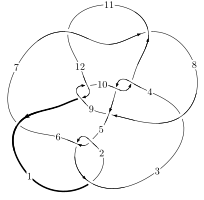
\includegraphics[width=112pt]{../../../GIT/diagram.site/Diagrams/png/1102_12a_0301.png}\\
\ \ \ A knot diagram\footnotemark}&
\allowdisplaybreaks
\textbf{Linearized knot diagam} \\
\cline{2-2}
 &
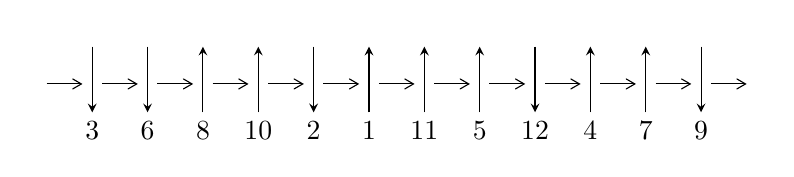
\begin{tikzpicture}[x=20pt, y=17pt]
	% nodes
	\node (C0) at (0, 0) {};
	\node (C1) at (1, 0) {};
	\node (C1U) at (1, +1) {};
	\node (C1D) at (1, -1) {3};

	\node (C2) at (2, 0) {};
	\node (C2U) at (2, +1) {};
	\node (C2D) at (2, -1) {6};

	\node (C3) at (3, 0) {};
	\node (C3U) at (3, +1) {};
	\node (C3D) at (3, -1) {8};

	\node (C4) at (4, 0) {};
	\node (C4U) at (4, +1) {};
	\node (C4D) at (4, -1) {10};

	\node (C5) at (5, 0) {};
	\node (C5U) at (5, +1) {};
	\node (C5D) at (5, -1) {2};

	\node (C6) at (6, 0) {};
	\node (C6U) at (6, +1) {};
	\node (C6D) at (6, -1) {1};

	\node (C7) at (7, 0) {};
	\node (C7U) at (7, +1) {};
	\node (C7D) at (7, -1) {11};

	\node (C8) at (8, 0) {};
	\node (C8U) at (8, +1) {};
	\node (C8D) at (8, -1) {5};

	\node (C9) at (9, 0) {};
	\node (C9U) at (9, +1) {};
	\node (C9D) at (9, -1) {12};

	\node (C10) at (10, 0) {};
	\node (C10U) at (10, +1) {};
	\node (C10D) at (10, -1) {4};

	\node (C11) at (11, 0) {};
	\node (C11U) at (11, +1) {};
	\node (C11D) at (11, -1) {7};

	\node (C12) at (12, 0) {};
	\node (C12U) at (12, +1) {};
	\node (C12D) at (12, -1) {9};
	\node (C13) at (13, 0) {};

	% arrows
	\draw[->,>={angle 60}]
	(C0) edge (C1) (C1) edge (C2) (C2) edge (C3) (C3) edge (C4) (C4) edge (C5) (C5) edge (C6) (C6) edge (C7) (C7) edge (C8) (C8) edge (C9) (C9) edge (C10) (C10) edge (C11) (C11) edge (C12) (C12) edge (C13) ;	\draw[->,>=stealth]
	(C1U) edge (C1D) (C2U) edge (C2D) (C3D) edge (C3U) (C4D) edge (C4U) (C5U) edge (C5D) (C6D) edge (C6U) (C7D) edge (C7U) (C8D) edge (C8U) (C9U) edge (C9D) (C10D) edge (C10U) (C11D) edge (C11U) (C12U) edge (C12D) ;
	\end{tikzpicture} \\
\hhline{~~} \\& 
\textbf{Solving Sequence} \\ \cline{2-2} 
 &
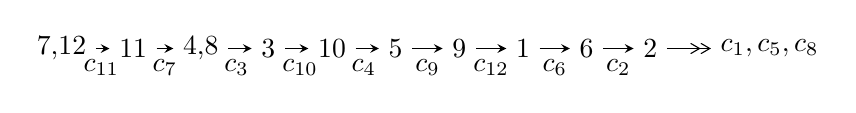
\begin{tikzpicture}[x=23pt, y=7pt]
	% node
	\node (A0) at (-1/8, 0) {7,12};
	\node (A1) at (1, 0) {11};
	\node (A2) at (33/16, 0) {4,8};
	\node (A3) at (25/8, 0) {3};
	\node (A4) at (33/8, 0) {10};
	\node (A5) at (41/8, 0) {5};
	\node (A6) at (49/8, 0) {9};
	\node (A7) at (57/8, 0) {1};
	\node (A8) at (65/8, 0) {6};
	\node (A9) at (73/8, 0) {2};
	\node (C1) at (1/2, -1) {$c_{11}$};
	\node (C2) at (3/2, -1) {$c_{7}$};
	\node (C3) at (21/8, -1) {$c_{3}$};
	\node (C4) at (29/8, -1) {$c_{10}$};
	\node (C5) at (37/8, -1) {$c_{4}$};
	\node (C6) at (45/8, -1) {$c_{9}$};
	\node (C7) at (53/8, -1) {$c_{12}$};
	\node (C8) at (61/8, -1) {$c_{6}$};
	\node (C9) at (69/8, -1) {$c_{2}$};
	\node (A10) at (11, 0) {$c_{1},c_{5},c_{8}$};

	% edge
	\draw[->,>=stealth]	
	(A0) edge (A1) (A1) edge (A2) (A2) edge (A3) (A3) edge (A4) (A4) edge (A5) (A5) edge (A6) (A6) edge (A7) (A7) edge (A8) (A8) edge (A9) ;
	\draw[->>,>={angle 60}]	
	(A9) edge (A10);
\end{tikzpicture} \\ 

\end{tabular} \\

\footnotetext{
The image of knot diagram is generated by the software ``\textbf{Draw programme}" developed by Andrew Bartholomew(\url{http://www.layer8.co.uk/maths/draw/index.htm\#Running-draw}), where we modified some parts for our purpose(\url{https://github.com/CATsTAILs/LinksPainter}).
}\phantom \\ \newline 
\centering \textbf{Ideals for irreducible components\footnotemark of $X_{\text{par}}$} 
 
\begin{align*}
I^u_{1}&=\langle 
-4.87061\times10^{819} u^{143}+1.43509\times10^{820} u^{142}+\cdots+1.18052\times10^{823} b+1.14666\times10^{826},\\
\phantom{I^u_{1}}&\phantom{= \langle  }4.47547\times10^{826} u^{143}-1.10984\times10^{827} u^{142}+\cdots+5.06813\times10^{829} a-2.27451\times10^{832},\\
\phantom{I^u_{1}}&\phantom{= \langle  }u^{144}-2 u^{143}+\cdots+43492785 u+4293137\rangle \\
I^u_{2}&=\langle 
-1449 u^{33}-2044 u^{32}+\cdots+b+83,\;1549 u^{33}+2128 u^{32}+\cdots+a-545,\;u^{34}+u^{33}+\cdots-6 u+1\rangle \\
\\
\end{align*}
\raggedright * 2 irreducible components of $\dim_{\mathbb{C}}=0$, with total 178 representations.\\
\footnotetext{All coefficients of polynomials are rational numbers. But the coefficients are sometimes approximated in decimal forms when there is not enough margin.}
\newpage
\renewcommand{\arraystretch}{1}
\centering \section*{I. $I^u_{1}= \langle -4.87\times10^{819} u^{143}+1.44\times10^{820} u^{142}+\cdots+1.18\times10^{823} b+1.15\times10^{826},\;4.48\times10^{826} u^{143}-1.11\times10^{827} u^{142}+\cdots+5.07\times10^{829} a-2.27\times10^{832},\;u^{144}-2 u^{143}+\cdots+43492785 u+4293137 \rangle$}
\flushleft \textbf{(i) Arc colorings}\\
\begin{tabular}{m{7pt} m{180pt} m{7pt} m{180pt} }
\flushright $a_{7}=$&$\begin{pmatrix}0\\u\end{pmatrix}$ \\
\flushright $a_{12}=$&$\begin{pmatrix}1\\0\end{pmatrix}$ \\
\flushright $a_{11}=$&$\begin{pmatrix}1\\u^2\end{pmatrix}$ \\
\flushright $a_{4}=$&$\begin{pmatrix}-0.000883062 u^{143}+0.00218985 u^{142}+\cdots+746.743 u+448.786\\0.000412583 u^{143}-0.00121564 u^{142}+\cdots-7800.84 u-971.315\end{pmatrix}$ \\
\flushright $a_{8}=$&$\begin{pmatrix}u\\u^3+u\end{pmatrix}$ \\
\flushright $a_{3}=$&$\begin{pmatrix}-0.000329909 u^{143}+0.000760842 u^{142}+\cdots-1701.22 u-34.1671\\0.000541090 u^{143}-0.00130988 u^{142}+\cdots+1411.66 u-68.8627\end{pmatrix}$ \\
\flushright $a_{10}=$&$\begin{pmatrix}-0.000383810 u^{143}+0.000957612 u^{142}+\cdots-872.514 u+74.6215\\0.000312112 u^{143}-0.000848011 u^{142}+\cdots-985.490 u-235.218\end{pmatrix}$ \\
\flushright $a_{5}=$&$\begin{pmatrix}-0.0000132490 u^{143}-0.000187625 u^{142}+\cdots-8836.60 u-904.601\\0.000163305 u^{143}-0.000487278 u^{142}+\cdots-3119.83 u-390.280\end{pmatrix}$ \\
\flushright $a_{9}=$&$\begin{pmatrix}-0.0000716976 u^{143}+0.000109602 u^{142}+\cdots-1858.00 u-160.596\\0.000312112 u^{143}-0.000848011 u^{142}+\cdots-985.490 u-235.218\end{pmatrix}$ \\
\flushright $a_{1}=$&$\begin{pmatrix}-0.000558490 u^{143}+0.00109744 u^{142}+\cdots-9944.74 u-773.191\\0.000391100 u^{143}-0.00112125 u^{142}+\cdots-4823.37 u-687.423\end{pmatrix}$ \\
\flushright $a_{6}=$&$\begin{pmatrix}0.000166748 u^{143}+0.000148454 u^{142}+\cdots+19122.8 u+1882.55\\-0.000808895 u^{143}+0.00189709 u^{142}+\cdots-4071.08 u-82.2661\end{pmatrix}$ \\
\flushright $a_{2}=$&$\begin{pmatrix}-0.000751067 u^{143}+0.00102591 u^{142}+\cdots-29590.0 u-2714.62\\0.000847809 u^{143}-0.00178305 u^{142}+\cdots+12346.0 u+921.364\end{pmatrix}$\\&\end{tabular}
\flushleft \textbf{(ii) Obstruction class $= -1$}\\~\\
\flushleft \textbf{(iii) Cusp Shapes $= 0.00103687 u^{143}-0.00285015 u^{142}+\cdots-12761.8 u-1827.63$}\\~\\
\newpage\renewcommand{\arraystretch}{1}
\flushleft \textbf{(iv) u-Polynomials at the component}\newline \\
\begin{tabular}{m{50pt}|m{274pt}}
Crossings & \hspace{64pt}u-Polynomials at each crossing \\
\hline $$\begin{aligned}c_{1}\end{aligned}$$&$\begin{aligned}
&u^{144}+73 u^{143}+\cdots+11 u+1
\end{aligned}$\\
\hline $$\begin{aligned}c_{2},c_{5}\end{aligned}$$&$\begin{aligned}
&u^{144}+3 u^{143}+\cdots+3 u+1
\end{aligned}$\\
\hline $$\begin{aligned}c_{3}\end{aligned}$$&$\begin{aligned}
&u^{144}+31 u^{142}+\cdots+1908503741 u+608565121
\end{aligned}$\\
\hline $$\begin{aligned}c_{4},c_{10}\end{aligned}$$&$\begin{aligned}
&u^{144}+u^{143}+\cdots+3922 u+11047
\end{aligned}$\\
\hline $$\begin{aligned}c_{6}\end{aligned}$$&$\begin{aligned}
&u^{144}+9 u^{143}+\cdots+5231795 u+492275
\end{aligned}$\\
\hline $$\begin{aligned}c_{7},c_{11}\end{aligned}$$&$\begin{aligned}
&u^{144}-2 u^{143}+\cdots+43492785 u+4293137
\end{aligned}$\\
\hline $$\begin{aligned}c_{8}\end{aligned}$$&$\begin{aligned}
&u^{144}-5 u^{143}+\cdots+323456 u+145664
\end{aligned}$\\
\hline $$\begin{aligned}c_{9},c_{12}\end{aligned}$$&$\begin{aligned}
&u^{144}-7 u^{143}+\cdots+448 u+241
\end{aligned}$\\
\hline
\end{tabular}\\~\\
\newpage\renewcommand{\arraystretch}{1}
\flushleft \textbf{(v) Riley Polynomials at the component}\newline \\
\begin{tabular}{m{50pt}|m{274pt}}
Crossings & \hspace{64pt}Riley Polynomials at each crossing \\
\hline $$\begin{aligned}c_{1}\end{aligned}$$&$\begin{aligned}
&y^{144}+7 y^{143}+\cdots+61 y+1
\end{aligned}$\\
\hline $$\begin{aligned}c_{2},c_{5}\end{aligned}$$&$\begin{aligned}
&y^{144}-73 y^{143}+\cdots-11 y+1
\end{aligned}$\\
\hline $$\begin{aligned}c_{3}\end{aligned}$$&$\begin{aligned}
&y^{144}+62 y^{143}+\cdots+1.71\times10^{19} y+3.70\times10^{17}
\end{aligned}$\\
\hline $$\begin{aligned}c_{4},c_{10}\end{aligned}$$&$\begin{aligned}
&y^{144}+99 y^{143}+\cdots+2246933046 y+122036209
\end{aligned}$\\
\hline $$\begin{aligned}c_{6}\end{aligned}$$&$\begin{aligned}
&y^{144}+59 y^{143}+\cdots+2859927161675 y+242334675625
\end{aligned}$\\
\hline $$\begin{aligned}c_{7},c_{11}\end{aligned}$$&$\begin{aligned}
&y^{144}+112 y^{143}+\cdots+363442723348927 y+18431025300769
\end{aligned}$\\
\hline $$\begin{aligned}c_{8}\end{aligned}$$&$\begin{aligned}
&y^{144}+21 y^{143}+\cdots+608957349888 y+21218000896
\end{aligned}$\\
\hline $$\begin{aligned}c_{9},c_{12}\end{aligned}$$&$\begin{aligned}
&y^{144}+81 y^{143}+\cdots+5275298 y+58081
\end{aligned}$\\
\hline
\end{tabular}\\~\\
\newpage\flushleft \textbf{(vi) Complex Volumes and Cusp Shapes}
$$\begin{array}{c|c|c}  
\text{Solutions to }I^u_{1}& \I (\text{vol} + \sqrt{-1}CS) & \text{Cusp shape}\\
 \hline 
\begin{aligned}
u &= \phantom{-}0.588974 + 0.806586 I \\
a &= \phantom{-}0.814707 + 0.212144 I \\
b &= -0.480786 + 0.038773 I\end{aligned}
 & \phantom{-}1.35258 + 1.78685 I & \phantom{-0.000000 } 0 \\ \hline\begin{aligned}
u &= \phantom{-}0.588974 - 0.806586 I \\
a &= \phantom{-}0.814707 - 0.212144 I \\
b &= -0.480786 - 0.038773 I\end{aligned}
 & \phantom{-}1.35258 - 1.78685 I & \phantom{-0.000000 } 0 \\ \hline\begin{aligned}
u &= \phantom{-}0.552108 + 0.839164 I \\
a &= -1.279280 - 0.047757 I \\
b &= \phantom{-}0.553192 - 0.358983 I\end{aligned}
 & -0.35099 - 2.68683 I & \phantom{-0.000000 } 0 \\ \hline\begin{aligned}
u &= \phantom{-}0.552108 - 0.839164 I \\
a &= -1.279280 + 0.047757 I \\
b &= \phantom{-}0.553192 + 0.358983 I\end{aligned}
 & -0.35099 + 2.68683 I & \phantom{-0.000000 } 0 \\ \hline\begin{aligned}
u &= \phantom{-}1.005370 + 0.062527 I \\
a &= \phantom{-}0.104281 - 0.381311 I \\
b &= \phantom{-}0.61943 - 1.48558 I\end{aligned}
 & \phantom{-}2.68193 - 5.85769 I & \phantom{-0.000000 } 0 \\ \hline\begin{aligned}
u &= \phantom{-}1.005370 - 0.062527 I \\
a &= \phantom{-}0.104281 + 0.381311 I \\
b &= \phantom{-}0.61943 + 1.48558 I\end{aligned}
 & \phantom{-}2.68193 + 5.85769 I & \phantom{-0.000000 } 0 \\ \hline\begin{aligned}
u &= -0.220365 + 0.993377 I \\
a &= \phantom{-}0.85710 + 2.02083 I \\
b &= -0.179134 - 0.769240 I\end{aligned}
 & -3.75668 - 2.02618 I & \phantom{-0.000000 } 0 \\ \hline\begin{aligned}
u &= -0.220365 - 0.993377 I \\
a &= \phantom{-}0.85710 - 2.02083 I \\
b &= -0.179134 + 0.769240 I\end{aligned}
 & -3.75668 + 2.02618 I & \phantom{-0.000000 } 0 \\ \hline\begin{aligned}
u &= \phantom{-}0.663510 + 0.714334 I \\
a &= -0.622284 + 0.116258 I \\
b &= \phantom{-}0.494383 - 0.205448 I\end{aligned}
 & -0.77640 - 2.27763 I & \phantom{-0.000000 } 0 \\ \hline\begin{aligned}
u &= \phantom{-}0.663510 - 0.714334 I \\
a &= -0.622284 - 0.116258 I \\
b &= \phantom{-}0.494383 + 0.205448 I\end{aligned}
 & -0.77640 + 2.27763 I & \phantom{-0.000000 } 0\\
 \hline 
 \end{array}$$\newpage$$\begin{array}{c|c|c}  
\text{Solutions to }I^u_{1}& \I (\text{vol} + \sqrt{-1}CS) & \text{Cusp shape}\\
 \hline 
\begin{aligned}
u &= -0.254448 + 1.004160 I \\
a &= \phantom{-}0.34549 + 3.18852 I \\
b &= \phantom{-}1.12753 - 2.12776 I\end{aligned}
 & -2.68755 - 9.48016 I & \phantom{-0.000000 } 0 \\ \hline\begin{aligned}
u &= -0.254448 - 1.004160 I \\
a &= \phantom{-}0.34549 - 3.18852 I \\
b &= \phantom{-}1.12753 + 2.12776 I\end{aligned}
 & -2.68755 + 9.48016 I & \phantom{-0.000000 } 0 \\ \hline\begin{aligned}
u &= \phantom{-}0.116003 + 1.031380 I \\
a &= -0.752872 + 0.148868 I \\
b &= \phantom{-}1.43735 + 0.44324 I\end{aligned}
 & -0.955085 - 0.942202 I & \phantom{-0.000000 } 0 \\ \hline\begin{aligned}
u &= \phantom{-}0.116003 - 1.031380 I \\
a &= -0.752872 - 0.148868 I \\
b &= \phantom{-}1.43735 - 0.44324 I\end{aligned}
 & -0.955085 + 0.942202 I & \phantom{-0.000000 } 0 \\ \hline\begin{aligned}
u &= \phantom{-}0.615971 + 0.853128 I \\
a &= \phantom{-}0.313127 + 0.522083 I \\
b &= -0.469295 - 0.339372 I\end{aligned}
 & \phantom{-}0.99262 + 2.96528 I & \phantom{-0.000000 } 0 \\ \hline\begin{aligned}
u &= \phantom{-}0.615971 - 0.853128 I \\
a &= \phantom{-}0.313127 - 0.522083 I \\
b &= -0.469295 + 0.339372 I\end{aligned}
 & \phantom{-}0.99262 - 2.96528 I & \phantom{-0.000000 } 0 \\ \hline\begin{aligned}
u &= \phantom{-}0.561725 + 0.758384 I \\
a &= \phantom{-}0.598946 - 0.063054 I \\
b &= -0.546435 - 0.015274 I\end{aligned}
 & \phantom{-}1.22604 + 1.75594 I & \phantom{-0.000000 } 0 \\ \hline\begin{aligned}
u &= \phantom{-}0.561725 - 0.758384 I \\
a &= \phantom{-}0.598946 + 0.063054 I \\
b &= -0.546435 + 0.015274 I\end{aligned}
 & \phantom{-}1.22604 - 1.75594 I & \phantom{-0.000000 } 0 \\ \hline\begin{aligned}
u &= -0.198296 + 1.043170 I \\
a &= \phantom{-}0.01554 - 3.00067 I \\
b &= -1.10648 + 2.07716 I\end{aligned}
 & -0.59723 - 4.65435 I & \phantom{-0.000000 } 0 \\ \hline\begin{aligned}
u &= -0.198296 - 1.043170 I \\
a &= \phantom{-}0.01554 + 3.00067 I \\
b &= -1.10648 - 2.07716 I\end{aligned}
 & -0.59723 + 4.65435 I & \phantom{-0.000000 } 0\\
 \hline 
 \end{array}$$\newpage$$\begin{array}{c|c|c}  
\text{Solutions to }I^u_{1}& \I (\text{vol} + \sqrt{-1}CS) & \text{Cusp shape}\\
 \hline 
\begin{aligned}
u &= \phantom{-}0.408176 + 0.981073 I \\
a &= -0.130120 + 0.354158 I \\
b &= \phantom{-}0.264137 - 0.428591 I\end{aligned}
 & -0.99525 + 2.97182 I & \phantom{-0.000000 } 0 \\ \hline\begin{aligned}
u &= \phantom{-}0.408176 - 0.981073 I \\
a &= -0.130120 - 0.354158 I \\
b &= \phantom{-}0.264137 + 0.428591 I\end{aligned}
 & -0.99525 - 2.97182 I & \phantom{-0.000000 } 0 \\ \hline\begin{aligned}
u &= \phantom{-}0.312845 + 1.028380 I \\
a &= -0.706686 + 0.112894 I \\
b &= \phantom{-}1.286400 + 0.151620 I\end{aligned}
 & -0.79795 + 6.14591 I & \phantom{-0.000000 } 0 \\ \hline\begin{aligned}
u &= \phantom{-}0.312845 - 1.028380 I \\
a &= -0.706686 - 0.112894 I \\
b &= \phantom{-}1.286400 - 0.151620 I\end{aligned}
 & -0.79795 - 6.14591 I & \phantom{-0.000000 } 0 \\ \hline\begin{aligned}
u &= -0.020124 + 1.077150 I \\
a &= \phantom{-}0.85194 - 2.59546 I \\
b &= -1.00450 + 1.92895 I\end{aligned}
 & \phantom{-}0.15992 - 2.69156 I & \phantom{-0.000000 } 0 \\ \hline\begin{aligned}
u &= -0.020124 - 1.077150 I \\
a &= \phantom{-}0.85194 + 2.59546 I \\
b &= -1.00450 - 1.92895 I\end{aligned}
 & \phantom{-}0.15992 + 2.69156 I & \phantom{-0.000000 } 0 \\ \hline\begin{aligned}
u &= \phantom{-}0.108232 + 1.075700 I \\
a &= -1.26822 + 2.17941 I \\
b &= \phantom{-}0.87786 - 1.76992 I\end{aligned}
 & -1.11315 + 2.01264 I & \phantom{-0.000000 } 0 \\ \hline\begin{aligned}
u &= \phantom{-}0.108232 - 1.075700 I \\
a &= -1.26822 - 2.17941 I \\
b &= \phantom{-}0.87786 + 1.76992 I\end{aligned}
 & -1.11315 - 2.01264 I & \phantom{-0.000000 } 0 \\ \hline\begin{aligned}
u &= \phantom{-}0.348479 + 0.841255 I \\
a &= \phantom{-}0.706723 - 0.049308 I \\
b &= -0.987714 - 0.269842 I\end{aligned}
 & \phantom{-}1.37682 + 2.28432 I & \phantom{-0.000000 } 0 \\ \hline\begin{aligned}
u &= \phantom{-}0.348479 - 0.841255 I \\
a &= \phantom{-}0.706723 + 0.049308 I \\
b &= -0.987714 + 0.269842 I\end{aligned}
 & \phantom{-}1.37682 - 2.28432 I & \phantom{-0.000000 } 0\\
 \hline 
 \end{array}$$\newpage$$\begin{array}{c|c|c}  
\text{Solutions to }I^u_{1}& \I (\text{vol} + \sqrt{-1}CS) & \text{Cusp shape}\\
 \hline 
\begin{aligned}
u &= \phantom{-}0.663458 + 0.872096 I \\
a &= -0.179121 - 0.657961 I \\
b &= \phantom{-}0.528871 + 0.517276 I\end{aligned}
 & -1.19337 + 7.42439 I & \phantom{-0.000000 } 0 \\ \hline\begin{aligned}
u &= \phantom{-}0.663458 - 0.872096 I \\
a &= -0.179121 + 0.657961 I \\
b &= \phantom{-}0.528871 - 0.517276 I\end{aligned}
 & -1.19337 - 7.42439 I & \phantom{-0.000000 } 0 \\ \hline\begin{aligned}
u &= -0.838504 + 0.318893 I \\
a &= -1.042270 - 0.444996 I \\
b &= -0.682946 - 0.959518 I\end{aligned}
 & -5.20423 - 7.14103 I & \phantom{-0.000000 } 0 \\ \hline\begin{aligned}
u &= -0.838504 - 0.318893 I \\
a &= -1.042270 + 0.444996 I \\
b &= -0.682946 + 0.959518 I\end{aligned}
 & -5.20423 + 7.14103 I & \phantom{-0.000000 } 0 \\ \hline\begin{aligned}
u &= -0.846408 + 0.238041 I \\
a &= \phantom{-}0.235642 + 1.272120 I \\
b &= \phantom{-}0.026187 + 0.955549 I\end{aligned}
 & \phantom{-}0.62706 + 8.26152 I & \phantom{-0.000000 } 0 \\ \hline\begin{aligned}
u &= -0.846408 - 0.238041 I \\
a &= \phantom{-}0.235642 - 1.272120 I \\
b &= \phantom{-}0.026187 - 0.955549 I\end{aligned}
 & \phantom{-}0.62706 - 8.26152 I & \phantom{-0.000000 } 0 \\ \hline\begin{aligned}
u &= -0.229432 + 1.100660 I \\
a &= -0.835734 - 0.058002 I \\
b &= -0.539507 + 0.372564 I\end{aligned}
 & \phantom{-}3.02392 - 4.18388 I & \phantom{-0.000000 } 0 \\ \hline\begin{aligned}
u &= -0.229432 - 1.100660 I \\
a &= -0.835734 + 0.058002 I \\
b &= -0.539507 - 0.372564 I\end{aligned}
 & \phantom{-}3.02392 + 4.18388 I & \phantom{-0.000000 } 0 \\ \hline\begin{aligned}
u &= -0.164064 + 1.120810 I \\
a &= \phantom{-}0.910405 + 0.394437 I \\
b &= \phantom{-}0.534511 - 0.463425 I\end{aligned}
 & \phantom{-}2.49148 + 1.82953 I & \phantom{-0.000000 } 0 \\ \hline\begin{aligned}
u &= -0.164064 - 1.120810 I \\
a &= \phantom{-}0.910405 - 0.394437 I \\
b &= \phantom{-}0.534511 + 0.463425 I\end{aligned}
 & \phantom{-}2.49148 - 1.82953 I & \phantom{-0.000000 } 0\\
 \hline 
 \end{array}$$\newpage$$\begin{array}{c|c|c}  
\text{Solutions to }I^u_{1}& \I (\text{vol} + \sqrt{-1}CS) & \text{Cusp shape}\\
 \hline 
\begin{aligned}
u &= \phantom{-}0.602181 + 0.962757 I \\
a &= -0.017523 - 0.464247 I \\
b &= \phantom{-}0.189249 + 0.582642 I\end{aligned}
 & -2.24076 + 0.35611 I & \phantom{-0.000000 } 0 \\ \hline\begin{aligned}
u &= \phantom{-}0.602181 - 0.962757 I \\
a &= -0.017523 + 0.464247 I \\
b &= \phantom{-}0.189249 - 0.582642 I\end{aligned}
 & -2.24076 - 0.35611 I & \phantom{-0.000000 } 0 \\ \hline\begin{aligned}
u &= -0.343761 + 0.784853 I \\
a &= -1.44286 - 1.89551 I \\
b &= -0.157834 + 0.299506 I\end{aligned}
 & -5.23945 - 6.83479 I & \phantom{-0.000000 } 0 \\ \hline\begin{aligned}
u &= -0.343761 - 0.784853 I \\
a &= -1.44286 + 1.89551 I \\
b &= -0.157834 - 0.299506 I\end{aligned}
 & -5.23945 + 6.83479 I & \phantom{-0.000000 } 0 \\ \hline\begin{aligned}
u &= -0.018942 + 1.149860 I \\
a &= \phantom{-}0.32580 + 1.83647 I \\
b &= -0.835072 - 0.860030 I\end{aligned}
 & -5.09191 + 0.88313 I & \phantom{-0.000000 } 0 \\ \hline\begin{aligned}
u &= -0.018942 - 1.149860 I \\
a &= \phantom{-}0.32580 - 1.83647 I \\
b &= -0.835072 + 0.860030 I\end{aligned}
 & -5.09191 - 0.88313 I & \phantom{-0.000000 } 0 \\ \hline\begin{aligned}
u &= -0.780566 + 0.251437 I \\
a &= -0.182848 - 1.298480 I \\
b &= \phantom{-}0.058926 - 0.906421 I\end{aligned}
 & \phantom{-}3.10843 + 3.24691 I & \phantom{-0.000000 } 0 \\ \hline\begin{aligned}
u &= -0.780566 - 0.251437 I \\
a &= -0.182848 + 1.298480 I \\
b &= \phantom{-}0.058926 + 0.906421 I\end{aligned}
 & \phantom{-}3.10843 - 3.24691 I & \phantom{-0.000000 } 0 \\ \hline\begin{aligned}
u &= -0.433416 + 0.692395 I \\
a &= -0.892030 + 0.420953 I \\
b &= \phantom{-}1.09657 + 1.30641 I\end{aligned}
 & -1.87167 + 6.68892 I & \phantom{-0.000000 } 0 \\ \hline\begin{aligned}
u &= -0.433416 - 0.692395 I \\
a &= -0.892030 - 0.420953 I \\
b &= \phantom{-}1.09657 - 1.30641 I\end{aligned}
 & -1.87167 - 6.68892 I & \phantom{-0.000000 } 0\\
 \hline 
 \end{array}$$\newpage$$\begin{array}{c|c|c}  
\text{Solutions to }I^u_{1}& \I (\text{vol} + \sqrt{-1}CS) & \text{Cusp shape}\\
 \hline 
\begin{aligned}
u &= \phantom{-}0.039597 + 1.187340 I \\
a &= -0.23079 - 1.72372 I \\
b &= \phantom{-}1.029770 + 0.840840 I\end{aligned}
 & -7.51047 + 6.26493 I & \phantom{-0.000000 } 0 \\ \hline\begin{aligned}
u &= \phantom{-}0.039597 - 1.187340 I \\
a &= -0.23079 + 1.72372 I \\
b &= \phantom{-}1.029770 - 0.840840 I\end{aligned}
 & -7.51047 - 6.26493 I & \phantom{-0.000000 } 0 \\ \hline\begin{aligned}
u &= \phantom{-}0.028137 + 0.810981 I \\
a &= \phantom{-}0.857357 - 0.120226 I \\
b &= -1.185570 - 0.689334 I\end{aligned}
 & \phantom{-}1.16811 + 2.58837 I & \phantom{-0.000000 } 0 \\ \hline\begin{aligned}
u &= \phantom{-}0.028137 - 0.810981 I \\
a &= \phantom{-}0.857357 + 0.120226 I \\
b &= -1.185570 + 0.689334 I\end{aligned}
 & \phantom{-}1.16811 - 2.58837 I & \phantom{-0.000000 } 0 \\ \hline\begin{aligned}
u &= \phantom{-}0.685639 + 0.398945 I \\
a &= -0.714999 + 0.142005 I \\
b &= \phantom{-}0.267849 - 0.158035 I\end{aligned}
 & -0.78982 + 4.43480 I & \phantom{-0.000000 } 0 \\ \hline\begin{aligned}
u &= \phantom{-}0.685639 - 0.398945 I \\
a &= -0.714999 - 0.142005 I \\
b &= \phantom{-}0.267849 + 0.158035 I\end{aligned}
 & -0.78982 - 4.43480 I & \phantom{-0.000000 } 0 \\ \hline\begin{aligned}
u &= -0.747504 + 0.180586 I \\
a &= \phantom{-}0.918151 + 0.133298 I \\
b &= \phantom{-}0.376430 + 1.020790 I\end{aligned}
 & -2.80400 - 2.61780 I & \phantom{-0.000000 } 0 \\ \hline\begin{aligned}
u &= -0.747504 - 0.180586 I \\
a &= \phantom{-}0.918151 - 0.133298 I \\
b &= \phantom{-}0.376430 - 1.020790 I\end{aligned}
 & -2.80400 + 2.61780 I & \phantom{-0.000000 } 0 \\ \hline\begin{aligned}
u &= -0.749959 + 0.113090 I \\
a &= \phantom{-}0.246223 + 1.375070 I \\
b &= -0.183531 + 1.054220 I\end{aligned}
 & -1.382460 + 0.261042 I & \phantom{-0.000000 } 0 \\ \hline\begin{aligned}
u &= -0.749959 - 0.113090 I \\
a &= \phantom{-}0.246223 - 1.375070 I \\
b &= -0.183531 - 1.054220 I\end{aligned}
 & -1.382460 - 0.261042 I & \phantom{-0.000000 } 0\\
 \hline 
 \end{array}$$\newpage$$\begin{array}{c|c|c}  
\text{Solutions to }I^u_{1}& \I (\text{vol} + \sqrt{-1}CS) & \text{Cusp shape}\\
 \hline 
\begin{aligned}
u &= \phantom{-}0.123292 + 1.235550 I \\
a &= -0.024057 + 0.397629 I \\
b &= \phantom{-}0.721977 - 0.549297 I\end{aligned}
 & -3.24642 + 2.41794 I & \phantom{-0.000000 } 0 \\ \hline\begin{aligned}
u &= \phantom{-}0.123292 - 1.235550 I \\
a &= -0.024057 - 0.397629 I \\
b &= \phantom{-}0.721977 + 0.549297 I\end{aligned}
 & -3.24642 - 2.41794 I & \phantom{-0.000000 } 0 \\ \hline\begin{aligned}
u &= \phantom{-}0.920219 + 0.847649 I \\
a &= -0.534998 + 0.453594 I \\
b &= -0.562416 + 0.175354 I\end{aligned}
 & -2.38529 + 3.49979 I & \phantom{-0.000000 } 0 \\ \hline\begin{aligned}
u &= \phantom{-}0.920219 - 0.847649 I \\
a &= -0.534998 - 0.453594 I \\
b &= -0.562416 - 0.175354 I\end{aligned}
 & -2.38529 - 3.49979 I & \phantom{-0.000000 } 0 \\ \hline\begin{aligned}
u &= -0.104504 + 1.246890 I \\
a &= -0.49877 - 1.67441 I \\
b &= \phantom{-}0.80656 + 1.23008 I\end{aligned}
 & -10.16430 - 2.09519 I & \phantom{-0.000000 } 0 \\ \hline\begin{aligned}
u &= -0.104504 - 1.246890 I \\
a &= -0.49877 + 1.67441 I \\
b &= \phantom{-}0.80656 - 1.23008 I\end{aligned}
 & -10.16430 + 2.09519 I & \phantom{-0.000000 } 0 \\ \hline\begin{aligned}
u &= -0.376709 + 1.207980 I \\
a &= \phantom{-}0.49740 + 2.08303 I \\
b &= \phantom{-}1.06246 - 2.02022 I\end{aligned}
 & -4.73479 - 2.67171 I & \phantom{-0.000000 } 0 \\ \hline\begin{aligned}
u &= -0.376709 - 1.207980 I \\
a &= \phantom{-}0.49740 - 2.08303 I \\
b &= \phantom{-}1.06246 + 2.02022 I\end{aligned}
 & -4.73479 + 2.67171 I & \phantom{-0.000000 } 0 \\ \hline\begin{aligned}
u &= -0.444938 + 1.190580 I \\
a &= -0.91678 - 1.72233 I \\
b &= -0.37710 + 1.79378 I\end{aligned}
 & -4.79129 - 6.15356 I & \phantom{-0.000000 } 0 \\ \hline\begin{aligned}
u &= -0.444938 - 1.190580 I \\
a &= -0.91678 + 1.72233 I \\
b &= -0.37710 - 1.79378 I\end{aligned}
 & -4.79129 + 6.15356 I & \phantom{-0.000000 } 0\\
 \hline 
 \end{array}$$\newpage$$\begin{array}{c|c|c}  
\text{Solutions to }I^u_{1}& \I (\text{vol} + \sqrt{-1}CS) & \text{Cusp shape}\\
 \hline 
\begin{aligned}
u &= -0.400594 + 1.209200 I \\
a &= -0.384054 + 0.146148 I \\
b &= -0.606258 + 0.194163 I\end{aligned}
 & \phantom{-}0.04470 - 7.58979 I & \phantom{-0.000000 } 0 \\ \hline\begin{aligned}
u &= -0.400594 - 1.209200 I \\
a &= -0.384054 - 0.146148 I \\
b &= -0.606258 - 0.194163 I\end{aligned}
 & \phantom{-}0.04470 + 7.58979 I & \phantom{-0.000000 } 0 \\ \hline\begin{aligned}
u &= \phantom{-}0.710136 + 0.117628 I \\
a &= -0.343029 + 0.215010 I \\
b &= -0.760564 + 1.115220 I\end{aligned}
 & \phantom{-}2.39029 - 1.41778 I & \phantom{-0.000000 } 0 \\ \hline\begin{aligned}
u &= \phantom{-}0.710136 - 0.117628 I \\
a &= -0.343029 - 0.215010 I \\
b &= -0.760564 - 1.115220 I\end{aligned}
 & \phantom{-}2.39029 + 1.41778 I & \phantom{-0.000000 } 0 \\ \hline\begin{aligned}
u &= -0.717147 + 0.015494 I \\
a &= \phantom{-}0.331720 - 0.326283 I \\
b &= \phantom{-}0.047403 - 1.201530 I\end{aligned}
 & -1.38519 + 1.85665 I & \phantom{-0.000000 } 0 \\ \hline\begin{aligned}
u &= -0.717147 - 0.015494 I \\
a &= \phantom{-}0.331720 + 0.326283 I \\
b &= \phantom{-}0.047403 + 1.201530 I\end{aligned}
 & -1.38519 - 1.85665 I & \phantom{-0.000000 } 0 \\ \hline\begin{aligned}
u &= -0.326609 + 1.258210 I \\
a &= \phantom{-}0.363087 - 0.010208 I \\
b &= \phantom{-}0.681362 - 0.244980 I\end{aligned}
 & -5.04746 - 4.10538 I & \phantom{-0.000000 } 0 \\ \hline\begin{aligned}
u &= -0.326609 - 1.258210 I \\
a &= \phantom{-}0.363087 + 0.010208 I \\
b &= \phantom{-}0.681362 + 0.244980 I\end{aligned}
 & -5.04746 + 4.10538 I & \phantom{-0.000000 } 0 \\ \hline\begin{aligned}
u &= \phantom{-}0.024138 + 1.299960 I \\
a &= -0.052500 - 0.354159 I \\
b &= -0.804034 + 0.514563 I\end{aligned}
 & -7.22328 - 1.44072 I & \phantom{-0.000000 } 0 \\ \hline\begin{aligned}
u &= \phantom{-}0.024138 - 1.299960 I \\
a &= -0.052500 + 0.354159 I \\
b &= -0.804034 - 0.514563 I\end{aligned}
 & -7.22328 + 1.44072 I & \phantom{-0.000000 } 0\\
 \hline 
 \end{array}$$\newpage$$\begin{array}{c|c|c}  
\text{Solutions to }I^u_{1}& \I (\text{vol} + \sqrt{-1}CS) & \text{Cusp shape}\\
 \hline 
\begin{aligned}
u &= -0.574477 + 0.398863 I \\
a &= \phantom{-}0.121276 - 1.349280 I \\
b &= \phantom{-}0.244153 - 0.686304 I\end{aligned}
 & \phantom{-}4.98422 + 1.09428 I & \phantom{-0.000000 } 0 \\ \hline\begin{aligned}
u &= -0.574477 - 0.398863 I \\
a &= \phantom{-}0.121276 + 1.349280 I \\
b &= \phantom{-}0.244153 + 0.686304 I\end{aligned}
 & \phantom{-}4.98422 - 1.09428 I & \phantom{-0.000000 } 0 \\ \hline\begin{aligned}
u &= -0.896813 + 0.949012 I \\
a &= -0.835360 - 1.133600 I \\
b &= -1.66185 + 0.17676 I\end{aligned}
 & -6.05078 - 0.28308 I & \phantom{-0.000000 } 0 \\ \hline\begin{aligned}
u &= -0.896813 - 0.949012 I \\
a &= -0.835360 + 1.133600 I \\
b &= -1.66185 - 0.17676 I\end{aligned}
 & -6.05078 + 0.28308 I & \phantom{-0.000000 } 0 \\ \hline\begin{aligned}
u &= -0.546921 + 0.424202 I \\
a &= -0.858030 + 0.658167 I \\
b &= \phantom{-}0.69435 + 1.35145 I\end{aligned}
 & -2.43049 - 0.79621 I & \phantom{-0.000000 } 0 \\ \hline\begin{aligned}
u &= -0.546921 - 0.424202 I \\
a &= -0.858030 - 0.658167 I \\
b &= \phantom{-}0.69435 - 1.35145 I\end{aligned}
 & -2.43049 + 0.79621 I & \phantom{-0.000000 } 0 \\ \hline\begin{aligned}
u &= -0.437988 + 1.243590 I \\
a &= \phantom{-}0.315246 - 0.162105 I \\
b &= \phantom{-}0.621025 - 0.144861 I\end{aligned}
 & -2.63906 - 12.95050 I & \phantom{-0.000000 } 0 \\ \hline\begin{aligned}
u &= -0.437988 - 1.243590 I \\
a &= \phantom{-}0.315246 + 0.162105 I \\
b &= \phantom{-}0.621025 + 0.144861 I\end{aligned}
 & -2.63906 + 12.95050 I & \phantom{-0.000000 } 0 \\ \hline\begin{aligned}
u &= \phantom{-}0.169686 + 1.310780 I \\
a &= \phantom{-}0.044715 - 0.352540 I \\
b &= -0.750252 + 0.627963 I\end{aligned}
 & -6.23195 + 7.10872 I & \phantom{-0.000000 } 0 \\ \hline\begin{aligned}
u &= \phantom{-}0.169686 - 1.310780 I \\
a &= \phantom{-}0.044715 + 0.352540 I \\
b &= -0.750252 - 0.627963 I\end{aligned}
 & -6.23195 - 7.10872 I & \phantom{-0.000000 } 0\\
 \hline 
 \end{array}$$\newpage$$\begin{array}{c|c|c}  
\text{Solutions to }I^u_{1}& \I (\text{vol} + \sqrt{-1}CS) & \text{Cusp shape}\\
 \hline 
\begin{aligned}
u &= -0.405777 + 0.484780 I \\
a &= -0.45411 + 1.38784 I \\
b &= -0.380910 + 0.594374 I\end{aligned}
 & \phantom{-}4.28423 - 3.95321 I & \phantom{-}8.83973 + 5.08072 I \\ \hline\begin{aligned}
u &= -0.405777 - 0.484780 I \\
a &= -0.45411 - 1.38784 I \\
b &= -0.380910 - 0.594374 I\end{aligned}
 & \phantom{-}4.28423 + 3.95321 I & \phantom{-}8.83973 - 5.08072 I \\ \hline\begin{aligned}
u &= -0.375711 + 1.318400 I \\
a &= \phantom{-}0.30255 + 1.85564 I \\
b &= \phantom{-}1.22831 - 2.05684 I\end{aligned}
 & -4.72511 - 2.68988 I & \phantom{-0.000000 } 0 \\ \hline\begin{aligned}
u &= -0.375711 - 1.318400 I \\
a &= \phantom{-}0.30255 - 1.85564 I \\
b &= \phantom{-}1.22831 + 2.05684 I\end{aligned}
 & -4.72511 + 2.68988 I & \phantom{-0.000000 } 0 \\ \hline\begin{aligned}
u &= \phantom{-}0.378389 + 1.327700 I \\
a &= -0.29232 + 1.78878 I \\
b &= -0.70586 - 1.75721 I\end{aligned}
 & -1.64399 + 5.55551 I & \phantom{-0.000000 } 0 \\ \hline\begin{aligned}
u &= \phantom{-}0.378389 - 1.327700 I \\
a &= -0.29232 - 1.78878 I \\
b &= -0.70586 + 1.75721 I\end{aligned}
 & -1.64399 - 5.55551 I & \phantom{-0.000000 } 0 \\ \hline\begin{aligned}
u &= -0.260086 + 0.557311 I \\
a &= \phantom{-}1.089100 - 0.374280 I \\
b &= -0.95277 - 1.07001 I\end{aligned}
 & \phantom{-}0.70399 + 2.55333 I & \phantom{-}2.39179 - 1.33477 I \\ \hline\begin{aligned}
u &= -0.260086 - 0.557311 I \\
a &= \phantom{-}1.089100 + 0.374280 I \\
b &= -0.95277 + 1.07001 I\end{aligned}
 & \phantom{-}0.70399 - 2.55333 I & \phantom{-}2.39179 + 1.33477 I \\ \hline\begin{aligned}
u &= \phantom{-}1.392090 + 0.059866 I \\
a &= -0.041688 + 0.516633 I \\
b &= \phantom{-}0.19444 + 2.15296 I\end{aligned}
 & \phantom{-}0.34432 + 7.14034 I & \phantom{-0.000000 } 0 \\ \hline\begin{aligned}
u &= \phantom{-}1.392090 - 0.059866 I \\
a &= -0.041688 - 0.516633 I \\
b &= \phantom{-}0.19444 - 2.15296 I\end{aligned}
 & \phantom{-}0.34432 - 7.14034 I & \phantom{-0.000000 } 0\\
 \hline 
 \end{array}$$\newpage$$\begin{array}{c|c|c}  
\text{Solutions to }I^u_{1}& \I (\text{vol} + \sqrt{-1}CS) & \text{Cusp shape}\\
 \hline 
\begin{aligned}
u &= -0.424343 + 1.331970 I \\
a &= -0.89922 - 1.51222 I \\
b &= \phantom{-}0.17293 + 2.13223 I\end{aligned}
 & -7.32112 - 7.04455 I & \phantom{-0.000000 } 0 \\ \hline\begin{aligned}
u &= -0.424343 - 1.331970 I \\
a &= -0.89922 + 1.51222 I \\
b &= \phantom{-}0.17293 - 2.13223 I\end{aligned}
 & -7.32112 + 7.04455 I & \phantom{-0.000000 } 0 \\ \hline\begin{aligned}
u &= -0.363811 + 1.365390 I \\
a &= \phantom{-}0.81478 + 1.48788 I \\
b &= -0.40176 - 2.05770 I\end{aligned}
 & -11.51500 - 3.54675 I & \phantom{-0.000000 } 0 \\ \hline\begin{aligned}
u &= -0.363811 - 1.365390 I \\
a &= \phantom{-}0.81478 - 1.48788 I \\
b &= -0.40176 + 2.05770 I\end{aligned}
 & -11.51500 + 3.54675 I & \phantom{-0.000000 } 0 \\ \hline\begin{aligned}
u &= \phantom{-}0.46535 + 1.35157 I \\
a &= \phantom{-}0.41281 - 1.73538 I \\
b &= \phantom{-}0.92905 + 1.88759 I\end{aligned}
 & -1.50949 + 11.08430 I & \phantom{-0.000000 } 0 \\ \hline\begin{aligned}
u &= \phantom{-}0.46535 - 1.35157 I \\
a &= \phantom{-}0.41281 + 1.73538 I \\
b &= \phantom{-}0.92905 - 1.88759 I\end{aligned}
 & -1.50949 - 11.08430 I & \phantom{-0.000000 } 0 \\ \hline\begin{aligned}
u &= -0.534256 + 0.175599 I \\
a &= -1.41161 + 0.75020 I \\
b &= -0.157668 - 0.785039 I\end{aligned}
 & -6.59405 + 0.21495 I & -8.07961 - 1.24156 I \\ \hline\begin{aligned}
u &= -0.534256 - 0.175599 I \\
a &= -1.41161 - 0.75020 I \\
b &= -0.157668 + 0.785039 I\end{aligned}
 & -6.59405 - 0.21495 I & -8.07961 + 1.24156 I \\ \hline\begin{aligned}
u &= -0.44954 + 1.36682 I \\
a &= \phantom{-}0.91887 + 1.45811 I \\
b &= -0.20940 - 2.27646 I\end{aligned}
 & -10.0795 - 11.8977 I & \phantom{-0.000000 } 0 \\ \hline\begin{aligned}
u &= -0.44954 - 1.36682 I \\
a &= \phantom{-}0.91887 - 1.45811 I \\
b &= -0.20940 + 2.27646 I\end{aligned}
 & -10.0795 + 11.8977 I & \phantom{-0.000000 } 0\\
 \hline 
 \end{array}$$\newpage$$\begin{array}{c|c|c}  
\text{Solutions to }I^u_{1}& \I (\text{vol} + \sqrt{-1}CS) & \text{Cusp shape}\\
 \hline 
\begin{aligned}
u &= \phantom{-}0.08155 + 1.44756 I \\
a &= \phantom{-}0.03237 + 1.48629 I \\
b &= \phantom{-}0.28223 - 1.84017 I\end{aligned}
 & -5.90985 + 2.79566 I & \phantom{-0.000000 } 0 \\ \hline\begin{aligned}
u &= \phantom{-}0.08155 - 1.44756 I \\
a &= \phantom{-}0.03237 - 1.48629 I \\
b &= \phantom{-}0.28223 + 1.84017 I\end{aligned}
 & -5.90985 - 2.79566 I & \phantom{-0.000000 } 0 \\ \hline\begin{aligned}
u &= \phantom{-}0.515683 + 0.191655 I \\
a &= \phantom{-}0.868388 - 0.149219 I \\
b &= -0.257523 + 0.044833 I\end{aligned}
 & \phantom{-}1.145010 + 0.395907 I & \phantom{-}8.43272 - 1.42917 I \\ \hline\begin{aligned}
u &= \phantom{-}0.515683 - 0.191655 I \\
a &= \phantom{-}0.868388 + 0.149219 I \\
b &= -0.257523 - 0.044833 I\end{aligned}
 & \phantom{-}1.145010 - 0.395907 I & \phantom{-}8.43272 + 1.42917 I \\ \hline\begin{aligned}
u &= -0.321300 + 0.441867 I \\
a &= -0.359364 + 1.057550 I \\
b &= \phantom{-}0.646998 + 0.435745 I\end{aligned}
 & -1.58511 - 1.03071 I & -2.17657 - 0.53205 I \\ \hline\begin{aligned}
u &= -0.321300 - 0.441867 I \\
a &= -0.359364 - 1.057550 I \\
b &= \phantom{-}0.646998 - 0.435745 I\end{aligned}
 & -1.58511 + 1.03071 I & -2.17657 + 0.53205 I \\ \hline\begin{aligned}
u &= -0.84358 + 1.19517 I \\
a &= \phantom{-}0.64702 + 1.26996 I \\
b &= \phantom{-}1.93434 - 0.86046 I\end{aligned}
 & -4.24592 - 3.74110 I & \phantom{-0.000000 } 0 \\ \hline\begin{aligned}
u &= -0.84358 - 1.19517 I \\
a &= \phantom{-}0.64702 - 1.26996 I \\
b &= \phantom{-}1.93434 + 0.86046 I\end{aligned}
 & -4.24592 + 3.74110 I & \phantom{-0.000000 } 0 \\ \hline\begin{aligned}
u &= \phantom{-}1.45129 + 0.25325 I \\
a &= \phantom{-}0.108702 - 0.526750 I \\
b &= \phantom{-}0.29191 - 2.13272 I\end{aligned}
 & -3.84358 + 3.69745 I & \phantom{-0.000000 } 0 \\ \hline\begin{aligned}
u &= \phantom{-}1.45129 - 0.25325 I \\
a &= \phantom{-}0.108702 + 0.526750 I \\
b &= \phantom{-}0.29191 + 2.13272 I\end{aligned}
 & -3.84358 - 3.69745 I & \phantom{-0.000000 } 0\\
 \hline 
 \end{array}$$\newpage$$\begin{array}{c|c|c}  
\text{Solutions to }I^u_{1}& \I (\text{vol} + \sqrt{-1}CS) & \text{Cusp shape}\\
 \hline 
\begin{aligned}
u &= \phantom{-}1.50001 + 0.01786 I \\
a &= \phantom{-}0.040577 - 0.552505 I \\
b &= -0.22698 - 2.42703 I\end{aligned}
 & -2.38759 + 12.01890 I & \phantom{-0.000000 } 0 \\ \hline\begin{aligned}
u &= \phantom{-}1.50001 - 0.01786 I \\
a &= \phantom{-}0.040577 + 0.552505 I \\
b &= -0.22698 + 2.42703 I\end{aligned}
 & -2.38759 - 12.01890 I & \phantom{-0.000000 } 0 \\ \hline\begin{aligned}
u &= -0.03046 + 1.50876 I \\
a &= -0.034479 - 1.355440 I \\
b &= -0.70117 + 1.92659 I\end{aligned}
 & -9.20997 - 2.44038 I & \phantom{-0.000000 } 0 \\ \hline\begin{aligned}
u &= -0.03046 - 1.50876 I \\
a &= -0.034479 + 1.355440 I \\
b &= -0.70117 - 1.92659 I\end{aligned}
 & -9.20997 + 2.44038 I & \phantom{-0.000000 } 0 \\ \hline\begin{aligned}
u &= \phantom{-}0.18707 + 1.54549 I \\
a &= \phantom{-}0.11795 - 1.47791 I \\
b &= -0.04073 + 2.24256 I\end{aligned}
 & -10.53950 + 6.99581 I & \phantom{-0.000000 } 0 \\ \hline\begin{aligned}
u &= \phantom{-}0.18707 - 1.54549 I \\
a &= \phantom{-}0.11795 + 1.47791 I \\
b &= -0.04073 - 2.24256 I\end{aligned}
 & -10.53950 - 6.99581 I & \phantom{-0.000000 } 0 \\ \hline\begin{aligned}
u &= \phantom{-}0.58892 + 1.45525 I \\
a &= \phantom{-}0.51439 - 1.57007 I \\
b &= \phantom{-}1.21400 + 2.25209 I\end{aligned}
 & -4.4747 + 13.8884 I & \phantom{-0.000000 } 0 \\ \hline\begin{aligned}
u &= \phantom{-}0.58892 - 1.45525 I \\
a &= \phantom{-}0.51439 + 1.57007 I \\
b &= \phantom{-}1.21400 - 2.25209 I\end{aligned}
 & -4.4747 - 13.8884 I & \phantom{-0.000000 } 0 \\ \hline\begin{aligned}
u &= \phantom{-}0.62506 + 1.47368 I \\
a &= -0.53986 + 1.53714 I \\
b &= -1.30785 - 2.32259 I\end{aligned}
 & -7.1676 + 19.1850 I & \phantom{-0.000000 } 0 \\ \hline\begin{aligned}
u &= \phantom{-}0.62506 - 1.47368 I \\
a &= -0.53986 - 1.53714 I \\
b &= -1.30785 + 2.32259 I\end{aligned}
 & -7.1676 - 19.1850 I & \phantom{-0.000000 } 0\\
 \hline 
 \end{array}$$\newpage$$\begin{array}{c|c|c}  
\text{Solutions to }I^u_{1}& \I (\text{vol} + \sqrt{-1}CS) & \text{Cusp shape}\\
 \hline 
\begin{aligned}
u &= \phantom{-}0.53960 + 1.50812 I \\
a &= -0.44875 + 1.53734 I \\
b &= -1.04384 - 2.37776 I\end{aligned}
 & -9.42147 + 10.38660 I & \phantom{-0.000000 } 0 \\ \hline\begin{aligned}
u &= \phantom{-}0.53960 - 1.50812 I \\
a &= -0.44875 - 1.53734 I \\
b &= -1.04384 + 2.37776 I\end{aligned}
 & -9.42147 - 10.38660 I & \phantom{-0.000000 } 0 \\ \hline\begin{aligned}
u &= -0.80497 + 1.43067 I \\
a &= \phantom{-}0.448147 + 1.301340 I \\
b &= \phantom{-}2.25308 - 1.49885 I\end{aligned}
 & -4.82162 - 3.73006 I & \phantom{-0.000000 } 0 \\ \hline\begin{aligned}
u &= -0.80497 - 1.43067 I \\
a &= \phantom{-}0.448147 - 1.301340 I \\
b &= \phantom{-}2.25308 + 1.49885 I\end{aligned}
 & -4.82162 + 3.73006 I & \phantom{-0.000000 } 0 \\ \hline\begin{aligned}
u &= -0.75952 + 1.59024 I \\
a &= -0.325959 - 1.292830 I \\
b &= -2.40942 + 1.95510 I\end{aligned}
 & -7.89532 - 0.16266 I & \phantom{-0.000000 } 0 \\ \hline\begin{aligned}
u &= -0.75952 - 1.59024 I \\
a &= -0.325959 + 1.292830 I \\
b &= -2.40942 - 1.95510 I\end{aligned}
 & -7.89532 + 0.16266 I & \phantom{-0.000000 } 0 \\ \hline\begin{aligned}
u &= -0.90874 + 1.51148 I \\
a &= -0.408405 - 1.217950 I \\
b &= -2.64198 + 1.51745 I\end{aligned}
 & -7.49720 - 7.84328 I & \phantom{-0.000000 } 0 \\ \hline\begin{aligned}
u &= -0.90874 - 1.51148 I \\
a &= -0.408405 + 1.217950 I \\
b &= -2.64198 - 1.51745 I\end{aligned}
 & -7.49720 + 7.84328 I & \phantom{-0.000000 } 0 \\ \hline\begin{aligned}
u &= \phantom{-}0.39392 + 1.75545 I \\
a &= -0.421747 + 1.209760 I \\
b &= -0.35466 - 3.04063 I\end{aligned}
 & -5.47321 + 0.58316 I & \phantom{-0.000000 } 0 \\ \hline\begin{aligned}
u &= \phantom{-}0.39392 - 1.75545 I \\
a &= -0.421747 - 1.209760 I \\
b &= -0.35466 + 3.04063 I\end{aligned}
 & -5.47321 - 0.58316 I & \phantom{-0.000000 } 0\\
 \hline 
 \end{array}$$\newpage$$\begin{array}{c|c|c}  
\text{Solutions to }I^u_{1}& \I (\text{vol} + \sqrt{-1}CS) & \text{Cusp shape}\\
 \hline 
\begin{aligned}
u &= \phantom{-}0.23900 + 1.88492 I \\
a &= \phantom{-}0.318729 - 1.242060 I \\
b &= -0.09185 + 3.52025 I\end{aligned}
 & -9.06744 - 3.79611 I & \phantom{-0.000000 } 0 \\ \hline\begin{aligned}
u &= \phantom{-}0.23900 - 1.88492 I \\
a &= \phantom{-}0.318729 + 1.242060 I \\
b &= -0.09185 - 3.52025 I\end{aligned}
 & -9.06744 + 3.79611 I & \phantom{-0.000000 } 0 \\ \hline\begin{aligned}
u &= \phantom{-}0.54878 + 1.88435 I \\
a &= \phantom{-}0.382473 - 1.120080 I \\
b &= \phantom{-}0.97041 + 3.35655 I\end{aligned}
 & -8.97505 + 5.09593 I & \phantom{-0.000000 } 0 \\ \hline\begin{aligned}
u &= \phantom{-}0.54878 - 1.88435 I \\
a &= \phantom{-}0.382473 + 1.120080 I \\
b &= \phantom{-}0.97041 - 3.35655 I\end{aligned}
 & -8.97505 - 5.09593 I & \phantom{-0.000000 } 0\\
 \hline 
 \end{array}$$\newpage\newpage\renewcommand{\arraystretch}{1}
\centering \section*{II. $I^u_{2}= \langle -1449 u^{33}-2044 u^{32}+\cdots+b+83,\;1549 u^{33}+2128 u^{32}+\cdots+a-545,\;u^{34}+u^{33}+\cdots-6 u+1 \rangle$}
\flushleft \textbf{(i) Arc colorings}\\
\begin{tabular}{m{7pt} m{180pt} m{7pt} m{180pt} }
\flushright $a_{7}=$&$\begin{pmatrix}0\\u\end{pmatrix}$ \\
\flushright $a_{12}=$&$\begin{pmatrix}1\\0\end{pmatrix}$ \\
\flushright $a_{11}=$&$\begin{pmatrix}1\\u^2\end{pmatrix}$ \\
\flushright $a_{4}=$&$\begin{pmatrix}-1549 u^{33}-2128 u^{32}+\cdots-5989 u+545\\1449 u^{33}+2044 u^{32}+\cdots+3796 u-83\end{pmatrix}$ \\
\flushright $a_{8}=$&$\begin{pmatrix}u\\u^3+u\end{pmatrix}$ \\
\flushright $a_{3}=$&$\begin{pmatrix}-754 u^{33}-679 u^{32}+\cdots-7675 u+1257\\2185 u^{33}+3143 u^{32}+\cdots+5239 u-25\end{pmatrix}$ \\
\flushright $a_{10}=$&$\begin{pmatrix}5 u^{32}+5 u^{31}+\cdots-238 u+57\\u^{33}+u^{32}+\cdots+32 u-6\end{pmatrix}$ \\
\flushright $a_{5}=$&$\begin{pmatrix}-220 u^{33}+130 u^{32}+\cdots-5587 u+1104\\787 u^{33}+345 u^{32}+\cdots+11042 u-1832\end{pmatrix}$ \\
\flushright $a_{9}=$&$\begin{pmatrix}u^{33}+6 u^{32}+\cdots-206 u+51\\u^{33}+u^{32}+\cdots+32 u-6\end{pmatrix}$ \\
\flushright $a_{1}=$&$\begin{pmatrix}51 u^{33}+50 u^{32}+\cdots+764 u-99\\-6 u^{33}-7 u^{32}+\cdots-83 u+4\end{pmatrix}$ \\
\flushright $a_{6}=$&$\begin{pmatrix}461 u^{33}+623 u^{32}+\cdots+1393 u+113\\-99 u^{33}-150 u^{32}+\cdots+185 u-170\end{pmatrix}$ \\
\flushright $a_{2}=$&$\begin{pmatrix}133 u^{33}+464 u^{32}+\cdots-4298 u+1015\\168 u^{33}+30 u^{32}+\cdots+4930 u-923\end{pmatrix}$\\&\end{tabular}
\flushleft \textbf{(ii) Obstruction class $= 1$}\\~\\
\flushleft \textbf{(iii) Cusp Shapes $= 917 u^{33}-1310 u^{32}+\cdots+34966 u-6672$}\\~\\
\newpage\renewcommand{\arraystretch}{1}
\flushleft \textbf{(iv) u-Polynomials at the component}\newline \\
\begin{tabular}{m{50pt}|m{274pt}}
Crossings & \hspace{64pt}u-Polynomials at each crossing \\
\hline $$\begin{aligned}c_{1}\end{aligned}$$&$\begin{aligned}
&u^{34}-18 u^{33}+\cdots-10 u+1
\end{aligned}$\\
\hline $$\begin{aligned}c_{2}\end{aligned}$$&$\begin{aligned}
&u^{34}+2 u^{33}+\cdots+2 u+1
\end{aligned}$\\
\hline $$\begin{aligned}c_{3}\end{aligned}$$&$\begin{aligned}
&u^{34}- u^{33}+\cdots+16 u^2+1
\end{aligned}$\\
\hline $$\begin{aligned}c_{4}\end{aligned}$$&$\begin{aligned}
&u^{34}+11 u^{32}+\cdots+3 u+1
\end{aligned}$\\
\hline $$\begin{aligned}c_{5}\end{aligned}$$&$\begin{aligned}
&u^{34}-2 u^{33}+\cdots-2 u+1
\end{aligned}$\\
\hline $$\begin{aligned}c_{6}\end{aligned}$$&$\begin{aligned}
&u^{34}-6 u^{33}+\cdots-4 u^2+1
\end{aligned}$\\
\hline $$\begin{aligned}c_{7}\end{aligned}$$&$\begin{aligned}
&u^{34}- u^{33}+\cdots+6 u+1
\end{aligned}$\\
\hline $$\begin{aligned}c_{8}\end{aligned}$$&$\begin{aligned}
&u^{34}+2 u^{32}+\cdots+3 u+1
\end{aligned}$\\
\hline $$\begin{aligned}c_{9}\end{aligned}$$&$\begin{aligned}
&u^{34}-6 u^{33}+\cdots+u+1
\end{aligned}$\\
\hline $$\begin{aligned}c_{10}\end{aligned}$$&$\begin{aligned}
&u^{34}+11 u^{32}+\cdots-3 u+1
\end{aligned}$\\
\hline $$\begin{aligned}c_{11}\end{aligned}$$&$\begin{aligned}
&u^{34}+u^{33}+\cdots-6 u+1
\end{aligned}$\\
\hline $$\begin{aligned}c_{12}\end{aligned}$$&$\begin{aligned}
&u^{34}+6 u^{33}+\cdots- u+1
\end{aligned}$\\
\hline
\end{tabular}\\~\\
\newpage\renewcommand{\arraystretch}{1}
\flushleft \textbf{(v) Riley Polynomials at the component}\newline \\
\begin{tabular}{m{50pt}|m{274pt}}
Crossings & \hspace{64pt}Riley Polynomials at each crossing \\
\hline $$\begin{aligned}c_{1}\end{aligned}$$&$\begin{aligned}
&y^{34}+6 y^{33}+\cdots+6 y+1
\end{aligned}$\\
\hline $$\begin{aligned}c_{2},c_{5}\end{aligned}$$&$\begin{aligned}
&y^{34}-18 y^{33}+\cdots-10 y+1
\end{aligned}$\\
\hline $$\begin{aligned}c_{3}\end{aligned}$$&$\begin{aligned}
&y^{34}+9 y^{33}+\cdots+32 y+1
\end{aligned}$\\
\hline $$\begin{aligned}c_{4},c_{10}\end{aligned}$$&$\begin{aligned}
&y^{34}+22 y^{33}+\cdots+27 y+1
\end{aligned}$\\
\hline $$\begin{aligned}c_{6}\end{aligned}$$&$\begin{aligned}
&y^{34}+6 y^{33}+\cdots-8 y+1
\end{aligned}$\\
\hline $$\begin{aligned}c_{7},c_{11}\end{aligned}$$&$\begin{aligned}
&y^{34}+31 y^{33}+\cdots+28 y+1
\end{aligned}$\\
\hline $$\begin{aligned}c_{8}\end{aligned}$$&$\begin{aligned}
&y^{34}+4 y^{33}+\cdots-19 y+1
\end{aligned}$\\
\hline $$\begin{aligned}c_{9},c_{12}\end{aligned}$$&$\begin{aligned}
&y^{34}+28 y^{33}+\cdots+31 y+1
\end{aligned}$\\
\hline
\end{tabular}\\~\\
\newpage\flushleft \textbf{(vi) Complex Volumes and Cusp Shapes}
$$\begin{array}{c|c|c}  
\text{Solutions to }I^u_{2}& \I (\text{vol} + \sqrt{-1}CS) & \text{Cusp shape}\\
 \hline 
\begin{aligned}
u &= \phantom{-}0.191167 + 1.022040 I \\
a &= \phantom{-}0.869542 - 0.392560 I \\
b &= \phantom{-}0.561024 + 0.524196 I\end{aligned}
 & \phantom{-}2.87251 - 2.10121 I & \phantom{-}7.29934 + 0. I\phantom{ +0.000000I} \\ \hline\begin{aligned}
u &= \phantom{-}0.191167 - 1.022040 I \\
a &= \phantom{-}0.869542 + 0.392560 I \\
b &= \phantom{-}0.561024 - 0.524196 I\end{aligned}
 & \phantom{-}2.87251 + 2.10121 I & \phantom{-}7.29934 + 0. I\phantom{ +0.000000I} \\ \hline\begin{aligned}
u &= \phantom{-}0.174005 + 0.941830 I \\
a &= -0.782482 - 0.069547 I \\
b &= -0.596449 - 0.432842 I\end{aligned}
 & \phantom{-}3.18425 + 3.55001 I & \phantom{-}2.36591 + 0. I\phantom{ +0.000000I} \\ \hline\begin{aligned}
u &= \phantom{-}0.174005 - 0.941830 I \\
a &= -0.782482 + 0.069547 I \\
b &= -0.596449 + 0.432842 I\end{aligned}
 & \phantom{-}3.18425 - 3.55001 I & \phantom{-}2.36591 + 0. I\phantom{ +0.000000I} \\ \hline\begin{aligned}
u &= \phantom{-}0.561343 + 0.931730 I \\
a &= -0.111886 - 0.393693 I \\
b &= \phantom{-}0.684926 - 0.211606 I\end{aligned}
 & -1.47095 + 2.36634 I & \phantom{-0.000000 } 0 \\ \hline\begin{aligned}
u &= \phantom{-}0.561343 - 0.931730 I \\
a &= -0.111886 + 0.393693 I \\
b &= \phantom{-}0.684926 + 0.211606 I\end{aligned}
 & -1.47095 - 2.36634 I & \phantom{-0.000000 } 0 \\ \hline\begin{aligned}
u &= -0.521603 + 0.957553 I \\
a &= \phantom{-}0.98747 + 1.93291 I \\
b &= \phantom{-}1.23742 - 0.81189 I\end{aligned}
 & -4.95756 - 7.76885 I & \phantom{-0.000000 } 0 \\ \hline\begin{aligned}
u &= -0.521603 - 0.957553 I \\
a &= \phantom{-}0.98747 - 1.93291 I \\
b &= \phantom{-}1.23742 + 0.81189 I\end{aligned}
 & -4.95756 + 7.76885 I & \phantom{-0.000000 } 0 \\ \hline\begin{aligned}
u &= \phantom{-}0.537317 + 0.632038 I \\
a &= \phantom{-}1.033360 - 0.110578 I \\
b &= \phantom{-}0.105202 + 1.258570 I\end{aligned}
 & -2.88749 + 1.16310 I & -4.11877 - 2.77849 I \\ \hline\begin{aligned}
u &= \phantom{-}0.537317 - 0.632038 I \\
a &= \phantom{-}1.033360 + 0.110578 I \\
b &= \phantom{-}0.105202 - 1.258570 I\end{aligned}
 & -2.88749 - 1.16310 I & -4.11877 + 2.77849 I\\
 \hline 
 \end{array}$$\newpage$$\begin{array}{c|c|c}  
\text{Solutions to }I^u_{2}& \I (\text{vol} + \sqrt{-1}CS) & \text{Cusp shape}\\
 \hline 
\begin{aligned}
u &= -0.472992 + 1.091720 I \\
a &= -0.64565 - 1.85526 I \\
b &= -1.14403 + 1.01661 I\end{aligned}
 & -3.30793 - 3.11279 I & \phantom{-0.000000 } 0 \\ \hline\begin{aligned}
u &= -0.472992 - 1.091720 I \\
a &= -0.64565 + 1.85526 I \\
b &= -1.14403 - 1.01661 I\end{aligned}
 & -3.30793 + 3.11279 I & \phantom{-0.000000 } 0 \\ \hline\begin{aligned}
u &= -0.767531 + 1.018810 I \\
a &= \phantom{-}0.96772 + 1.36100 I \\
b &= \phantom{-}1.60609 - 0.80485 I\end{aligned}
 & -6.29487 - 1.24377 I & \phantom{-0.000000 } 0 \\ \hline\begin{aligned}
u &= -0.767531 - 1.018810 I \\
a &= \phantom{-}0.96772 - 1.36100 I \\
b &= \phantom{-}1.60609 + 0.80485 I\end{aligned}
 & -6.29487 + 1.24377 I & \phantom{-0.000000 } 0 \\ \hline\begin{aligned}
u &= \phantom{-}0.400691 + 0.593368 I \\
a &= -0.833120 + 1.004930 I \\
b &= -0.584286 - 1.206530 I\end{aligned}
 & \phantom{-}0.93308 + 4.04917 I & \phantom{-}4.14785 - 6.31643 I \\ \hline\begin{aligned}
u &= \phantom{-}0.400691 - 0.593368 I \\
a &= -0.833120 - 1.004930 I \\
b &= -0.584286 + 1.206530 I\end{aligned}
 & \phantom{-}0.93308 - 4.04917 I & \phantom{-}4.14785 + 6.31643 I \\ \hline\begin{aligned}
u &= \phantom{-}0.108881 + 0.699899 I \\
a &= \phantom{-}1.062960 - 0.679577 I \\
b &= -1.042570 - 0.437362 I\end{aligned}
 & \phantom{-}0.98679 + 1.47341 I & -0.75167 + 2.47418 I \\ \hline\begin{aligned}
u &= \phantom{-}0.108881 - 0.699899 I \\
a &= \phantom{-}1.062960 + 0.679577 I \\
b &= -1.042570 + 0.437362 I\end{aligned}
 & \phantom{-}0.98679 - 1.47341 I & -0.75167 - 2.47418 I \\ \hline\begin{aligned}
u &= \phantom{-}0.430156 + 0.535349 I \\
a &= \phantom{-}1.44991 - 1.09036 I \\
b &= \phantom{-}0.56793 + 1.42993 I\end{aligned}
 & -1.43696 + 8.71820 I & \phantom{-}0.52151 - 8.82845 I \\ \hline\begin{aligned}
u &= \phantom{-}0.430156 - 0.535349 I \\
a &= \phantom{-}1.44991 + 1.09036 I \\
b &= \phantom{-}0.56793 - 1.42993 I\end{aligned}
 & -1.43696 - 8.71820 I & \phantom{-}0.52151 + 8.82845 I\\
 \hline 
 \end{array}$$\newpage$$\begin{array}{c|c|c}  
\text{Solutions to }I^u_{2}& \I (\text{vol} + \sqrt{-1}CS) & \text{Cusp shape}\\
 \hline 
\begin{aligned}
u &= \phantom{-}0.245797 + 0.610656 I \\
a &= \phantom{-}0.699203 + 1.193170 I \\
b &= -0.992414 - 0.902442 I\end{aligned}
 & \phantom{-}1.91035 + 2.96084 I & \phantom{-}8.91302 - 7.38262 I \\ \hline\begin{aligned}
u &= \phantom{-}0.245797 - 0.610656 I \\
a &= \phantom{-}0.699203 - 1.193170 I \\
b &= -0.992414 + 0.902442 I\end{aligned}
 & \phantom{-}1.91035 - 2.96084 I & \phantom{-}8.91302 + 7.38262 I \\ \hline\begin{aligned}
u &= \phantom{-}0.114888 + 0.626503 I \\
a &= -1.98668 + 0.21523 I \\
b &= \phantom{-}1.220040 + 0.554147 I\end{aligned}
 & -0.10391 + 4.93722 I & \phantom{-}1.75205 - 4.82134 I \\ \hline\begin{aligned}
u &= \phantom{-}0.114888 - 0.626503 I \\
a &= -1.98668 - 0.21523 I \\
b &= \phantom{-}1.220040 - 0.554147 I\end{aligned}
 & -0.10391 - 4.93722 I & \phantom{-}1.75205 + 4.82134 I \\ \hline\begin{aligned}
u &= \phantom{-}0.188919 + 0.577484 I \\
a &= -1.71516 - 1.32876 I \\
b &= \phantom{-}1.20718 + 0.85022 I\end{aligned}
 & \phantom{-}0.359771 - 1.188750 I & \phantom{-}5.16537 + 0.04112 I \\ \hline\begin{aligned}
u &= \phantom{-}0.188919 - 0.577484 I \\
a &= -1.71516 + 1.32876 I \\
b &= \phantom{-}1.20718 - 0.85022 I\end{aligned}
 & \phantom{-}0.359771 + 1.188750 I & \phantom{-}5.16537 - 0.04112 I \\ \hline\begin{aligned}
u &= -0.80963 + 1.27004 I \\
a &= -0.62953 - 1.28658 I \\
b &= -1.89479 + 1.24301 I\end{aligned}
 & -4.89455 - 3.88983 I & \phantom{-0.000000 } 0 \\ \hline\begin{aligned}
u &= -0.80963 - 1.27004 I \\
a &= -0.62953 + 1.28658 I \\
b &= -1.89479 - 1.24301 I\end{aligned}
 & -4.89455 + 3.88983 I & \phantom{-0.000000 } 0 \\ \hline\begin{aligned}
u &= -0.29394 + 1.56496 I \\
a &= -0.134365 - 1.396210 I \\
b &= -0.60597 + 2.19166 I\end{aligned}
 & -5.20461 - 1.85850 I & \phantom{-0.000000 } 0 \\ \hline\begin{aligned}
u &= -0.29394 - 1.56496 I \\
a &= -0.134365 + 1.396210 I \\
b &= -0.60597 - 2.19166 I\end{aligned}
 & -5.20461 + 1.85850 I & \phantom{-0.000000 } 0\\
 \hline 
 \end{array}$$\newpage$$\begin{array}{c|c|c}  
\text{Solutions to }I^u_{2}& \I (\text{vol} + \sqrt{-1}CS) & \text{Cusp shape}\\
 \hline 
\begin{aligned}
u &= -0.09200 + 1.71224 I \\
a &= \phantom{-}0.040387 + 1.269270 I \\
b &= -0.10955 - 2.60577 I\end{aligned}
 & -8.48052 + 2.96135 I & \phantom{-0.000000 } 0 \\ \hline\begin{aligned}
u &= -0.09200 - 1.71224 I \\
a &= \phantom{-}0.040387 - 1.269270 I \\
b &= -0.10955 + 2.60577 I\end{aligned}
 & -8.48052 - 2.96135 I & \phantom{-0.000000 } 0 \\ \hline\begin{aligned}
u &= -0.49547 + 1.77508 I \\
a &= \phantom{-}0.228343 + 1.257210 I \\
b &= \phantom{-}1.28025 - 2.87303 I\end{aligned}
 & -9.04089 - 5.96767 I & \phantom{-0.000000 } 0 \\ \hline\begin{aligned}
u &= -0.49547 - 1.77508 I \\
a &= \phantom{-}0.228343 - 1.257210 I \\
b &= \phantom{-}1.28025 + 2.87303 I\end{aligned}
 & -9.04089 + 5.96767 I & \phantom{-0.000000 } 0\\
 \hline 
 \end{array}$$\newpage
\newpage\renewcommand{\arraystretch}{1}
\centering \section*{ III. u-Polynomials}
\begin{tabular}{m{50pt}|m{274pt}}
Crossings & \hspace{64pt}u-Polynomials at each crossing \\
\hline $$\begin{aligned}c_{1}\end{aligned}$$&$\begin{aligned}
&(u^{34}-18 u^{33}+\cdots-10 u+1)(u^{144}+73 u^{143}+\cdots+11 u+1)
\end{aligned}$\\
\hline $$\begin{aligned}c_{2}\end{aligned}$$&$\begin{aligned}
&(u^{34}+2 u^{33}+\cdots+2 u+1)(u^{144}+3 u^{143}+\cdots+3 u+1)
\end{aligned}$\\
\hline $$\begin{aligned}c_{3}\end{aligned}$$&$\begin{aligned}
&(u^{34}- u^{33}+\cdots+16 u^2+1)\\
&\cdot(u^{144}+31 u^{142}+\cdots+1908503741 u+608565121)
\end{aligned}$\\
\hline $$\begin{aligned}c_{4}\end{aligned}$$&$\begin{aligned}
&(u^{34}+11 u^{32}+\cdots+3 u+1)(u^{144}+u^{143}+\cdots+3922 u+11047)
\end{aligned}$\\
\hline $$\begin{aligned}c_{5}\end{aligned}$$&$\begin{aligned}
&(u^{34}-2 u^{33}+\cdots-2 u+1)(u^{144}+3 u^{143}+\cdots+3 u+1)
\end{aligned}$\\
\hline $$\begin{aligned}c_{6}\end{aligned}$$&$\begin{aligned}
&(u^{34}-6 u^{33}+\cdots-4 u^2+1)(u^{144}+9 u^{143}+\cdots+5231795 u+492275)
\end{aligned}$\\
\hline $$\begin{aligned}c_{7}\end{aligned}$$&$\begin{aligned}
&(u^{34}- u^{33}+\cdots+6 u+1)(u^{144}-2 u^{143}+\cdots+4.34928\times10^{7} u+4293137)
\end{aligned}$\\
\hline $$\begin{aligned}c_{8}\end{aligned}$$&$\begin{aligned}
&(u^{34}+2 u^{32}+\cdots+3 u+1)(u^{144}-5 u^{143}+\cdots+323456 u+145664)
\end{aligned}$\\
\hline $$\begin{aligned}c_{9}\end{aligned}$$&$\begin{aligned}
&(u^{34}-6 u^{33}+\cdots+u+1)(u^{144}-7 u^{143}+\cdots+448 u+241)
\end{aligned}$\\
\hline $$\begin{aligned}c_{10}\end{aligned}$$&$\begin{aligned}
&(u^{34}+11 u^{32}+\cdots-3 u+1)(u^{144}+u^{143}+\cdots+3922 u+11047)
\end{aligned}$\\
\hline $$\begin{aligned}c_{11}\end{aligned}$$&$\begin{aligned}
&(u^{34}+u^{33}+\cdots-6 u+1)(u^{144}-2 u^{143}+\cdots+4.34928\times10^{7} u+4293137)
\end{aligned}$\\
\hline $$\begin{aligned}c_{12}\end{aligned}$$&$\begin{aligned}
&(u^{34}+6 u^{33}+\cdots- u+1)(u^{144}-7 u^{143}+\cdots+448 u+241)
\end{aligned}$\\
\hline
\end{tabular}\newpage\renewcommand{\arraystretch}{1}
\centering \section*{ IV. Riley Polynomials}
\begin{tabular}{m{50pt}|m{274pt}}
Crossings & \hspace{64pt}Riley Polynomials at each crossing \\
\hline $$\begin{aligned}c_{1}\end{aligned}$$&$\begin{aligned}
&(y^{34}+6 y^{33}+\cdots+6 y+1)(y^{144}+7 y^{143}+\cdots+61 y+1)
\end{aligned}$\\
\hline $$\begin{aligned}c_{2},c_{5}\end{aligned}$$&$\begin{aligned}
&(y^{34}-18 y^{33}+\cdots-10 y+1)(y^{144}-73 y^{143}+\cdots-11 y+1)
\end{aligned}$\\
\hline $$\begin{aligned}c_{3}\end{aligned}$$&$\begin{aligned}
&(y^{34}+9 y^{33}+\cdots+32 y+1)\\
&\cdot(y^{144}+62 y^{143}+\cdots+1.71\times10^{19} y+3.70\times10^{17})
\end{aligned}$\\
\hline $$\begin{aligned}c_{4},c_{10}\end{aligned}$$&$\begin{aligned}
&(y^{34}+22 y^{33}+\cdots+27 y+1)\\
&\cdot(y^{144}+99 y^{143}+\cdots+2246933046 y+122036209)
\end{aligned}$\\
\hline $$\begin{aligned}c_{6}\end{aligned}$$&$\begin{aligned}
&(y^{34}+6 y^{33}+\cdots-8 y+1)\\
&\cdot(y^{144}+59 y^{143}+\cdots+2859927161675 y+242334675625)
\end{aligned}$\\
\hline $$\begin{aligned}c_{7},c_{11}\end{aligned}$$&$\begin{aligned}
&(y^{34}+31 y^{33}+\cdots+28 y+1)\\
&\cdot(y^{144}+112 y^{143}+\cdots+363442723348927 y+18431025300769)
\end{aligned}$\\
\hline $$\begin{aligned}c_{8}\end{aligned}$$&$\begin{aligned}
&(y^{34}+4 y^{33}+\cdots-19 y+1)\\
&\cdot(y^{144}+21 y^{143}+\cdots+608957349888 y+21218000896)
\end{aligned}$\\
\hline $$\begin{aligned}c_{9},c_{12}\end{aligned}$$&$\begin{aligned}
&(y^{34}+28 y^{33}+\cdots+31 y+1)\\
&\cdot(y^{144}+81 y^{143}+\cdots+5275298 y+58081)
\end{aligned}$\\
\hline
\end{tabular}
\vskip 2pc
\end{document}